\section{Statement of research problem}
The utilization of renewable energy resources (RES) is on the rise, as many countries are making efforts to transition away from non-renewable energy sources due to their contribution to carbon emissions in the atmosphere. Microgrids combine distributed energy resources, energy storage, and load management. They have found applications in electrifying off-grid rural villages and remote regions. DC Microgrids (DCMG) have gained widespread use in aerospace, automotive, marine, and other industries. They serve as crucial components for integrating DERs (Distributed Energy Resources), especially since most renewable energy sources generate DC power. A nano grid, on the other hand, is designed for power distribution in a single house or small building [1]. A DC nano grid typically includes DERs, MPPT (Maximum Power Point Tracking), and ESS (Energy Storage System).\par
The use of renewable energy resources (RES) continues to grow. Numerous nations are seeking to transition from non-renewable energy sources as a result of the carbon emissions released into the atmosphere. A microgrid combines distributed energy resources, energy storage, and load. They have been used in the electrification of off-grid rural villages and remote areas. DC Microgrids (DCMG) have been widely used in aerospace, automotive, marine, and other industries. They are the critical components in integrating DERs since most renewable energies produced are in DC form. A nano grid is a power distribution system for a single house/small building. A DC nano grid consists of a DER, MPPT, and ESS.\par

\begin{figure}[H]
	\centering
	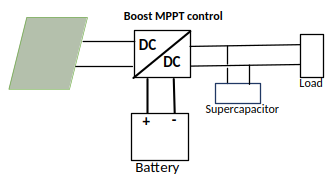
\includegraphics[totalheight=6cm]{Figures/dc nano grid.png}
	\caption{DC nano grid}
%	\label{fig:verticalcell}
\end{figure}
Nano grids are connected to form a microgrid cluster. The units in a microgrid can share resources. When the resources are shared in a Microgrid, substantial load variations and changes in generating capacity and storage will occur. In order to guarantee a stable Microgrid, a control system is required to maintain bus voltage at a constant level for as long as possible when load demand exceeds generation.\\\relax

\section{Background to the research problem}
Intermittency of Renewable Energy Sources (RES) poses a significant challenge in standalone DC Microgrids (DCMG). Additionally, variations in load, changes in generating and storage capacities, and unstable bus voltages further complicate microgrid stability. DCMGs are characterized by power-sharing, where Energy Resources (ERs) are distributed across the grid and connected via a bus line. DC-DC converters are essential components, adjusting source voltages to match the bus voltage.\par

In residential distribution systems (RDS), such as those using DERs like PV panels, load demand varies considerably based on usage, necessitating generation and load forecasting to manage these fluctuations effectively. The intermittency of RES adds complexity, making it challenging to manage constant load removal, power supply, and the balance between power production and demand. Hence, there's a clear need for a robust Energy Management System (EMS).\par

An EMS offers centralized and monitoring and control of energy usage across building systems, capable of recording, storing, and processing power consumption data from major household and industrial appliances. This research proposes an agent-based energy management system, which, when employed in a DC microgrid, can achieve a fully automated and stable grid with plug-and-play capabilities. Hierarchical control in a DC microgrid enhances grid efficiency by introducing load-shedding and minimizing downtime.\par

\section{Objectives of the research problem}
This research will mainly benefit communities in areas that experience severe power outages as a result of old failing infrastructure and utilities not being able to meet the ever-increasing energy demand. Energy management systems can help improve the robustness of microgrids ensuring that the grid remains stable and operational for a long time when energy is very limited.  Implementing DC microgrids in residential areas presents unique technical challenges that require specific solutions. Studies have been conducted for the energy management and control of DC microgrid systems for many reasons including power flow management, voltage regulation, and load balancing, to ensure reliable and efficient operation. The control strategies vary depending on MG structure; AC, DC [2]  or hybrid also the communication between the units [3].  This study aims to provide insights into integration of Distributed energy resources into residential areas with the focus on DC MG optimisation by resource sharing algorithm. 

\section{Delimitation of study}
This study does not cover the AC interface of a DC microgrid. AC-DC interface requires rectifications, usage of Active Front End (AFE) and special Topologies [4]. Therefore, the microgrid will fully operate in islanded mode. protection systems and devices are inherently more challenging, and the typical loads in residential buildings are not yet compatible with dc voltages. [5]. Protection systems are not discussed in this paper.

\section{Research Methodology}
The methodology employed in this study is primarily quantitative. Input data parameters are processed through a Matlab simulation model, allowing for comprehensive analysis. Software simulations are conducted to determine optimal system parameters, and these simulations involve the creation of a simulated model of a DC microgrid using computer software.\par
Within this simulated model, various parameters, mainly the battery state of charge (SoC), temperature, irradiance and load demand are systematically adjusted to create different scenarios and assess their impact on the grid's performance. These scenarios are designed to represent a range of potential real-world conditions and challenges.\par
Furthermore, to complement the digital simulations and provide real-life validation, a physical representation of the DC Microgrid (DC MG) is constructed. This physical system allows for hands-on analysis and experimentation, facilitating a deeper understanding of the data generated in the simulation phase.The combination of digital simulation and physical experimentation ensures a comprehensive and robust assessment of the DC microgrid's behavior and performance under varying conditions.

\subsection{Research Design}
The DC microgrid Energy Management System proposed in this paper is based on the Systems of Systems. Figure 2 shows four houses connected to the CGMS (Central Grid Management System). Each house is represented by a block in the Matlab Simulink model. These four houses represent four different scenarios serving as input parameters for the CGMS.

\subsubsection{Residential unit types}
\begin{enumerate}[nolistsep]
	\item A node with a storage system capable of both storing and sourcing energy for the microgrid.
	\item A node with only a storage system, without the capability to source energy.
	\item A node without a storage system, able to source energy only when sunlight is available.
	\item A node on the system that neither stores nor sources energy.
\end{enumerate}

The blocks are combined to form a microgrid that connects to the CGMS.
\begin{figure}[H]
	\centering
	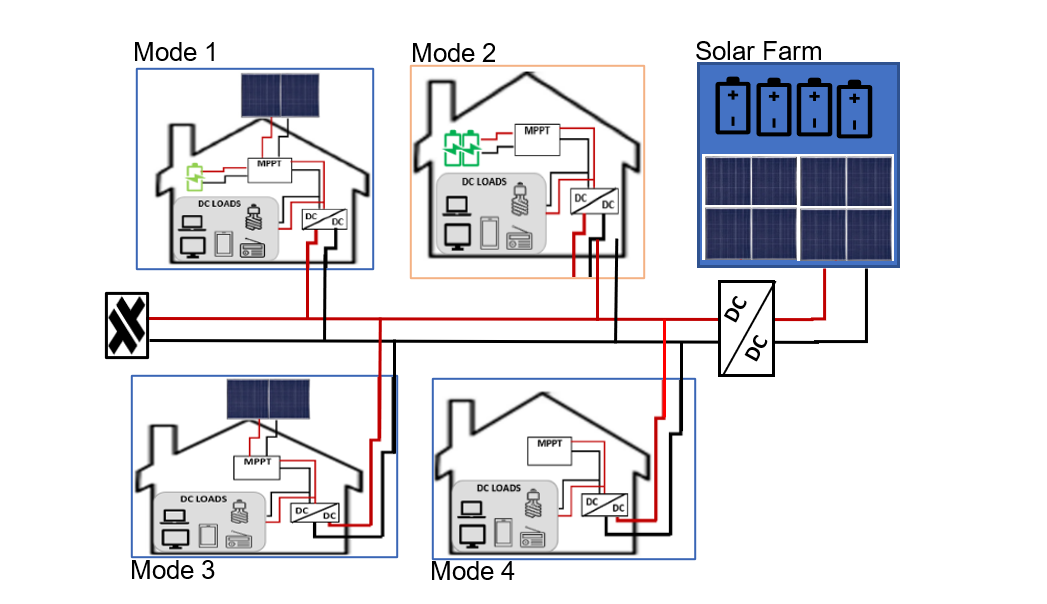
\includegraphics[totalheight=8cm]{Figures/re dc mg.png}
	\caption{esidential unit operation modes. (Mode 1) distributed generation and Energy storage. (Mode 2) energy storage only.}
	%	\label{fig:verticalcell}
\end{figure}
Nano grids are connected to form a microgrid cluster. The units in a microgrid can share resources. When the resources are shared in a Microgrid, substantial load variations and changes in generating capacity and storage will occur. In order to guarantee a stable Microgrid, a control system is required to maintain bus voltage at a constant level for as long as possible when load demand exceeds generation.

\subsection{Component technology.}
DC microgrid systems utilize renewable energy technologies like Photovoltaic (PV) modules and wind turbines. Among these, PV modules are particularly common and readily available at affordable prices for consumers. In this research, PV modules will be exclusively employed as the energy source.\par
The primary objective of this study is to test the energy management system algorithm under various scenarios. This will be achieved by adjusting the system's resources in a manner that triggers all possible operating states. Specifically, energy storage capacity and loads will vary for each unit tested.\par

\subsection{Simulation and optimisation}
The performance of the designed DC microgrid is modeled and simulated using Matlab/Simulink software. The simulation results are utilized to optimize system configurations, control strategies, and component sizing. This process aids in identifying potential improvements, evaluating system resilience, and validating the design.
\subsubsection{Software parameters required for load shedding regulation include:}
\begin{enumerate}
	\item Defining Load Sizes: Since each household may have different loads connected to the system, and considering the limited grid energy, an algorithm will be developed to determine the allowable power consumption for each household based on their contribution.
	\item State-of-Charge (SoC): SoC is a crucial parameter describing the remaining capacity of a battery. It is essential to monitor SoC during battery discharge to ensure efficient energy management.
	\item PV Irradiance Input: Irradiance levels vary with weather and day/night conditions. This parameter provides information about the available solar energy that can be used to charge the batteries.
	\item Connecting and Disconnecting of Loads: The system must be able to detect and react to changes, recalculating load shedding when significant loads are connected or disconnected.
\end{enumerate}
\subsection{Implementation}
A DC MG test bed will be constructed as described, incorporating key components such as DERs, energy storage systems, power converters, and control systems.


